% fig_ex_stage.tex - ex_stage (rtl/ex_stage.sv): operand muxes, ALU, branch unit,
% pc+imm adder, jalr target and the redirect decision sent back to if_stage.
\documentclass[tikz,border=8pt]{standalone}
\usepackage[T1]{fontenc}
\usepackage{lmodern}
\usepackage[scaled=0.92]{helvet}
\renewcommand{\familydefault}{\sfdefault}
% rv32i_style.tex - shared TikZ styles for the single-cycle RV32I diagrams.
% Visual language (same as the course PDF):
%   thick border, blue fill  = holds state (clocked)
%   thin border, white fill  = combinational logic
%   green trapezium          = multiplexer (0/1 marks the input chosen by select)
%   dashed orange            = control signal;  solid navy = data
%   /32 on a wire            = bus width;       dot = wires joined
% Port names are the exact SystemVerilog port names of the module drawn.
\usetikzlibrary{arrows.meta, positioning, calc, fit, backgrounds, shapes.geometric, shapes.misc}

\definecolor{ink}{RGB}{31,56,100}
\definecolor{statefill}{RGB}{220,230,242}
\definecolor{muxdraw}{RGB}{56,118,59}
\definecolor{muxfill}{RGB}{226,239,218}
\definecolor{ctrl}{RGB}{197,90,17}
\definecolor{ctrlfill}{RGB}{252,232,216}
\definecolor{note}{RGB}{110,110,110}
\definecolor{tintIF}{RGB}{236,243,251}
\definecolor{tintID}{RGB}{240,247,235}
\definecolor{tintEX}{RGB}{255,246,229}
\definecolor{tintMEM}{RGB}{244,237,249}
\definecolor{tintWB}{RGB}{233,246,245}

\tikzset{
  >={Stealth[length=2.2mm,width=1.6mm]},
  wire/.style      = {draw=ink, line width=0.75pt},
  data/.style      = {wire, ->},
  ctl/.style       = {draw=ctrl, line width=0.75pt, dashed, dash pattern=on 3pt off 1.6pt, ->},
  ctlnoarrow/.style= {draw=ctrl, line width=0.75pt, dashed, dash pattern=on 3pt off 1.6pt},
  block/.style     = {draw=ink, line width=0.75pt, fill=white, rectangle, align=center,
                      inner sep=3pt, font=\small},
  state/.style     = {block, line width=1.8pt, fill=statefill},
  ctrlblock/.style = {block, draw=ctrl, fill=ctrlfill},
  muxst/.style     = {draw=muxdraw, fill=muxfill, line width=0.9pt},
  aluSt/.style     = {draw=ink, fill=white, line width=0.9pt},
  addr/.style      = {circle, draw=ink, fill=white, line width=0.75pt, inner sep=0.5pt,
                      minimum size=6.5mm, font=\large},
  stage/.style     = {draw=ink!70, rounded corners=6pt, line width=0.9pt},
  sig/.style       = {font=\scriptsize\ttfamily, text=ink, inner sep=1.2pt},
  csig/.style      = {font=\scriptsize\ttfamily, text=ctrl, inner sep=1.2pt},
  wlbl/.style      = {font=\tiny, text=ink, inner sep=0.8pt},
  notetxt/.style   = {font=\scriptsize\itshape, text=note, align=left},
  mlbl/.style      = {font=\tiny\bfseries, text=muxdraw, inner sep=0pt},
  title/.style     = {font=\large\bfseries, text=ink},
  dot/.style       = {circle, fill=ink, inner sep=0pt, minimum size=4pt},
  cdot/.style      = {circle, fill=ctrl, inner sep=0pt, minimum size=4pt},
  portbox/.style   = {rectangle, fill=ink, inner sep=0pt, minimum size=4pt},
  cportbox/.style  = {rectangle, fill=ctrl, inner sep=0pt, minimum size=4pt},
  flag/.style      = {sig, draw=ink, fill=white, rounded corners=1.5pt, inner sep=1.5pt},  % net label
  stub/.style      = {ctl},                                                                 % named select input
}

% Two-line block label: module name, then "instance : module".
\newcommand{\blk}[2]{\textbf{#1}\\[-1pt]{\scriptsize\ttfamily #2}}
% Same with a two-line name.
\newcommand{\blkII}[3]{\textbf{#1}\\[-2pt]\textbf{#2}\\[-1pt]{\scriptsize\ttfamily #3}}

% Bus-width mark on a horizontal wire: \wmark{(x,y)}{32}
\newcommand{\wmark}[2]{%
  \draw[draw=ink, line width=0.6pt] ($#1+(-0.07,-0.13)$) -- ($#1+(0.07,0.13)$);
  \node[wlbl, above] at ($#1+(0,0.1)$) {#2};}
% Bus-width mark on a vertical wire: \wmarkv{(x,y)}{32}
\newcommand{\wmarkv}[2]{%
  \draw[draw=ink, line width=0.6pt] ($#1+(-0.13,-0.07)$) -- ($#1+(0.13,0.07)$);
  \node[wlbl, right] at ($#1+(0.1,0)$) {#2};}

% Multiplexer, inputs on the left, output on the right.
% \muxR{name}{x}{y}{height}: defines (name-out), (name-top), (name-bot), (name-l) (left x).
\newcommand{\muxR}[4]{%
  \draw[muxst] ($(#2,#3)+(-0.28,-#4/2)$) -- ($(#2,#3)+(-0.28,#4/2)$)
               -- ($(#2,#3)+(0.28,#4/2-0.28)$) -- ($(#2,#3)+(0.28,-#4/2+0.28)$) -- cycle;
  \coordinate (#1-out) at ($(#2,#3)+(0.28,0)$);
  \coordinate (#1-top) at ($(#2,#3)+(0,#4/2-0.14)$);
  \coordinate (#1-bot) at ($(#2,#3)+(0,-#4/2+0.14)$);
  \coordinate (#1-l)   at ($(#2,#3)+(-0.28,0)$);}

% ALU shape (notched trapezium), inputs a (upper) and b (lower) on the left.
% \aluR{name}{x}{y}{height}: defines (name-a), (name-b), (name-out), (name-op) (top edge).
\newcommand{\aluR}[4]{%
  \draw[aluSt] ($(#2,#3)+(-0.65,#4/2)$) -- ($(#2,#3)+(0.65,#4/4)$) -- ($(#2,#3)+(0.65,-#4/4)$)
               -- ($(#2,#3)+(-0.65,-#4/2)$) -- ($(#2,#3)+(-0.65,-0.28)$) -- ($(#2,#3)+(-0.35,0)$)
               -- ($(#2,#3)+(-0.65,0.28)$) -- cycle;
  \coordinate (#1-a)   at ($(#2,#3)+(-0.65,#4*0.3)$);
  \coordinate (#1-b)   at ($(#2,#3)+(-0.65,-#4*0.3)$);
  \coordinate (#1-out) at ($(#2,#3)+(0.65,0)$);
  \coordinate (#1-op)  at ($(#2,#3)+(0,#4*0.375)$);
  \coordinate (#1-c)   at ($(#2,#3)+(0.12,0)$);}

% Ports on a stage boundary. \inport{x}{y}{name}{width}  (label to the left)
% The width may be empty (1-bit port); it is expanded first so \foreach variables work.
\newcommand{\portw}[1]{\edef\pwtmp{#1}\ifx\pwtmp\empty\else\,[\pwtmp]\fi}
\newcommand{\inport}[4]{%
  \node[portbox] at (#1,#2) {};
  \node[sig, anchor=east] at ($(#1,#2)+(-0.12,0)$) {#3\portw{#4}};}
\newcommand{\cinport}[4]{%
  \node[cportbox] at (#1,#2) {};
  \node[csig, anchor=east] at ($(#1,#2)+(-0.12,0)$) {#3\portw{#4}};}
\newcommand{\outport}[4]{%
  \node[portbox] at (#1,#2) {};
  \node[sig, anchor=west] at ($(#1,#2)+(0.12,0)$) {#3\portw{#4}};}
\newcommand{\coutport}[4]{%
  \node[cportbox] at (#1,#2) {};
  \node[csig, anchor=west] at ($(#1,#2)+(0.12,0)$) {#3\portw{#4}};}
% Control input port on the top edge (label above).
\newcommand{\ctopport}[4]{%
  \node[cportbox] at (#1,#2) {};
  \node[csig, anchor=south] at ($(#1,#2)+(0,0.1)$) {#3\portw{#4}};}
% Data input port on the top edge (label above).
\newcommand{\topport}[4]{%
  \node[portbox] at (#1,#2) {};
  \node[sig, anchor=south] at ($(#1,#2)+(0,0.1)$) {#3\portw{#4}};}

% Legend strip. \legend{x}{y}
\newcommand{\legend}[2]{%
  \begin{scope}[shift={(#1,#2)}, font=\scriptsize]
    \node[state, minimum width=6mm, minimum height=3.5mm, inner sep=0pt] at (0,0) {};
    \node[anchor=west] at (0.45,0) {holds state};
    \node[block, minimum width=6mm, minimum height=3.5mm, inner sep=0pt] at (3.2,0) {};
    \node[anchor=west] at (3.65,0) {combinational};
    \draw[muxst] (6.2,-0.25) -- (6.2,0.25) -- (6.5,0.1) -- (6.5,-0.1) -- cycle;
    \node[anchor=west] at (6.6,0) {multiplexer};
    \draw[data] (8.7,0) -- (9.4,0); \node[anchor=west] at (9.45,0) {data};
    \draw[ctl] (10.4,0) -- (11.1,0); \node[anchor=west] at (11.15,0) {control};
    \node[portbox] at (12.6,0) {}; \node[anchor=west] at (12.7,0) {module port};
    \draw[wire] (14.6,0) -- (15.3,0); \draw[draw=ink, line width=0.6pt] (14.88,-0.13) -- (15.02,0.13);
    \node[wlbl] at (14.95,0.24) {32}; \node[anchor=west] at (15.35,0) {bus width};
  \end{scope}}

\begin{document}
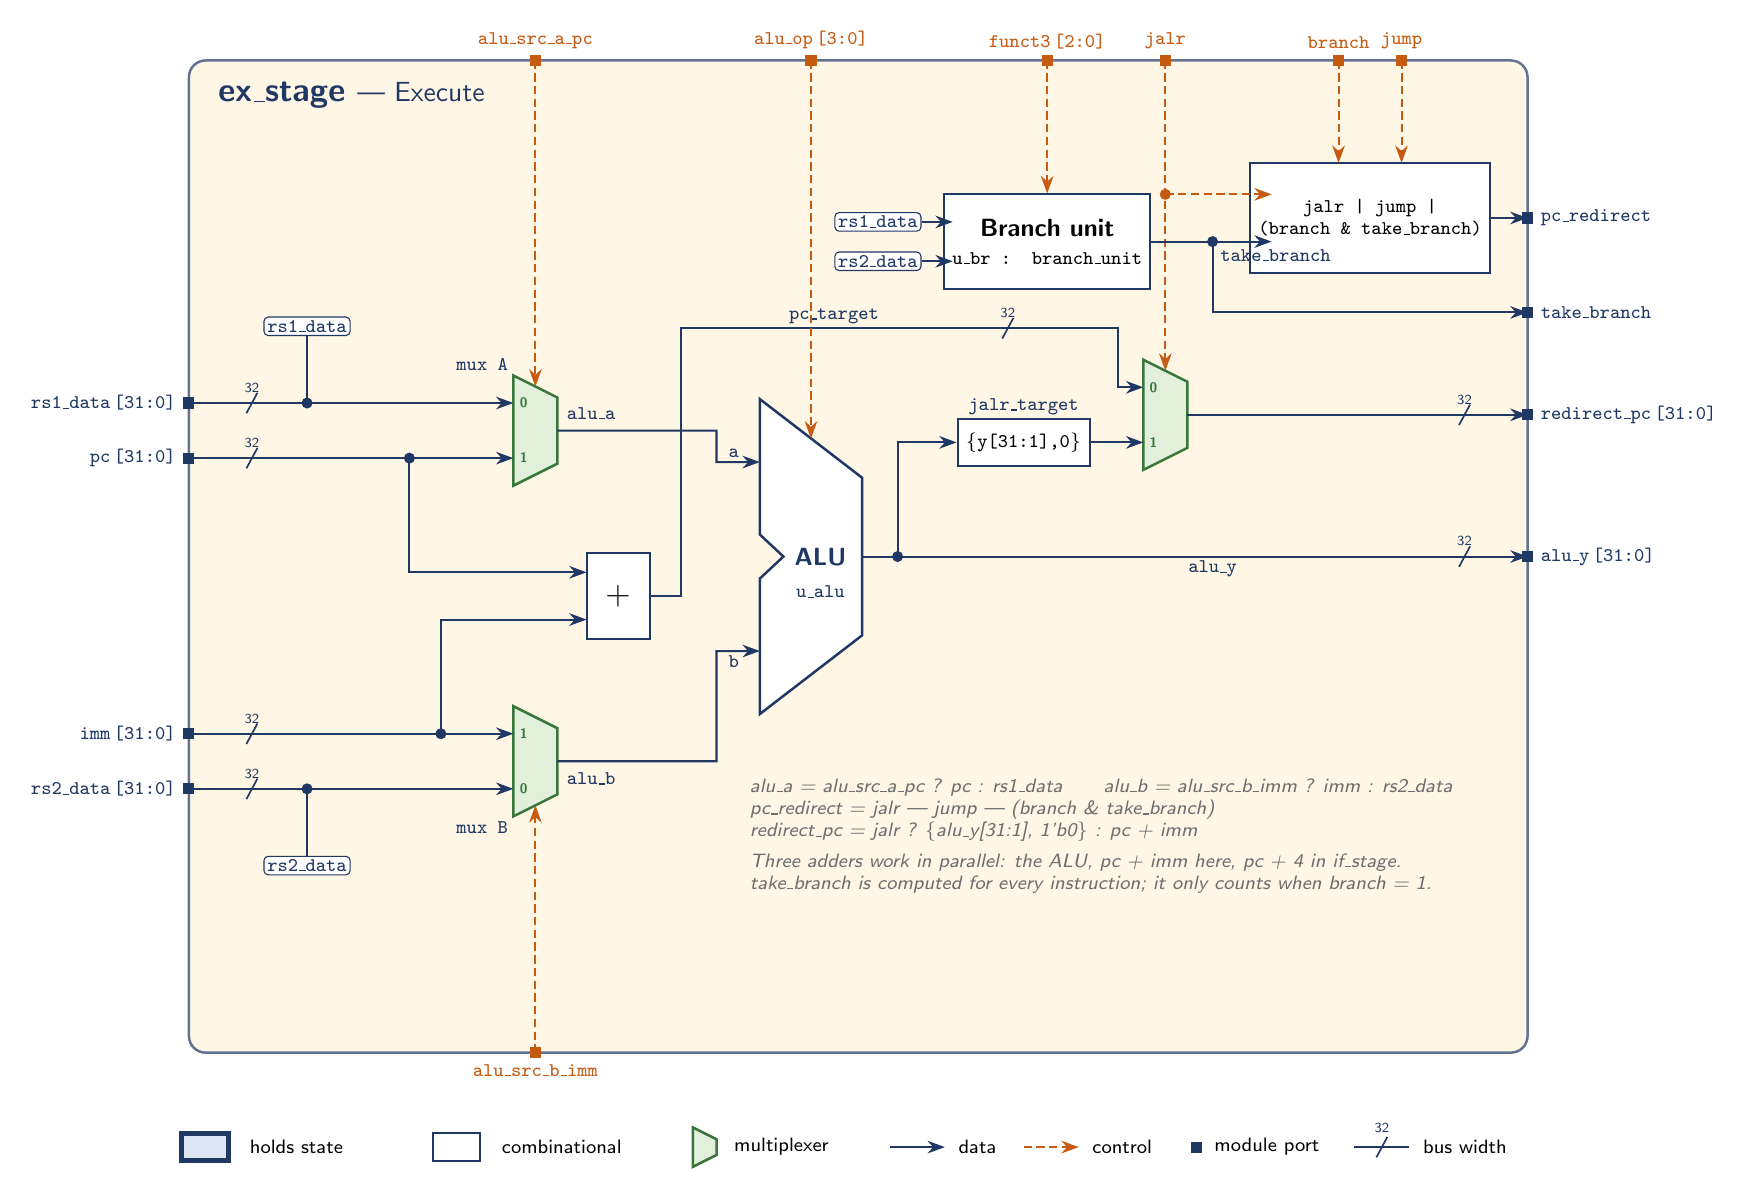
\begin{tikzpicture}
  % ---- stage boundary ----
  \draw[stage, fill=tintEX] (0,0) rectangle (17,12.6);
  \node[title, anchor=north west] at (0.25,12.45) {ex\_stage \textmd{\normalsize --- Execute}};

  % ---- ports ----
  \inport{0}{8.25}{rs1\_data}{31:0}
  \inport{0}{7.55}{pc}{31:0}
  \inport{0}{4.05}{imm}{31:0}
  \inport{0}{3.35}{rs2\_data}{31:0}
  \ctopport{4.4}{12.6}{alu\_src\_a\_pc}{}
  \ctopport{7.9}{12.6}{alu\_op}{3:0}
  \ctopport{10.9}{12.6}{funct3}{2:0}
  \ctopport{12.4}{12.6}{jalr}{}
  \ctopport{14.6}{12.6}{branch}{}
  \ctopport{15.4}{12.6}{jump}{}
  \node[cportbox] at (4.4,0) {};
  \node[csig, anchor=north] at (4.4,-0.1) {alu\_src\_b\_imm};
  \outport{17}{10.6}{pc\_redirect}{}
  \outport{17}{9.4}{take\_branch}{}
  \outport{17}{8.1}{redirect\_pc}{31:0}
  \outport{17}{6.3}{alu\_y}{31:0}

  % ---- operand muxes ----
  \muxR{ma}{4.4}{7.9}{1.4}
  \node[mlbl] at (4.25,8.25) {0};
  \node[mlbl] at (4.25,7.55) {1};
  \node[sig, anchor=south east] at (4.1,8.62) {mux A};
  \muxR{mb}{4.4}{3.7}{1.4}
  \node[mlbl] at (4.25,4.05) {1};
  \node[mlbl] at (4.25,3.35) {0};
  \node[sig, anchor=north east] at (4.1,2.98) {mux B};
  \draw[data] (0,8.25) -- (4.12,8.25);
  \draw[data] (0,7.55) -- (4.12,7.55);
  \draw[data] (0,4.05) -- (4.12,4.05);
  \draw[data] (0,3.35) -- (4.12,3.35);
  \draw[ctl] (4.4,12.6) -- (ma-top);
  \draw[ctl] (4.4,0) -- (mb-bot);

  % ---- pc + imm adder (branch / jal target) ----
  \node[block, minimum width=8mm, minimum height=11mm, font=\large] (add) at (5.45,5.8) {+};
  \node[dot] at (2.8,7.55) {};
  \draw[data] (2.8,7.55) -- (2.8,6.1) -- (5.05,6.1);
  \node[dot] at (3.2,4.05) {};
  \draw[data] (3.2,4.05) -- (3.2,5.5) -- (5.05,5.5);
  \draw[data] (add.east) -- (6.25,5.8) -- (6.25,9.2) -- node[sig, above, pos=0.35] {pc\_target} (11.8,9.2)
              -- (11.8,8.45) -- (12.12,8.45);

  % ---- ALU ----
  \aluR{alu}{7.9}{6.3}{4.0}
  \node[font=\bfseries\small, text=ink] at (alu-c) {ALU};
  \node[sig] at ($(alu-c)+(0,-0.45)$) {u\_alu};
  \draw[data] (ma-out) -- (6.7,7.9) -- (6.7,7.5) -- node[sig, above, pos=0.4] {a} (alu-a);
  \draw[data] (mb-out) -- (6.7,3.7) -- (6.7,5.1) -- node[sig, below, pos=0.4] {b} (alu-b);
  \node[sig, anchor=west] at (4.75,8.12) {alu\_a};
  \node[sig, anchor=west] at (4.75,3.48) {alu\_b};
  \draw[ctl] (7.9,12.6) -- (alu-op);
  \draw[wire] (alu-out) -- (9.0,6.3);
  \node[dot] at (9.0,6.3) {};
  \draw[data] (9.0,6.3) -- node[sig, below, pos=0.5] {alu\_y} (17,6.3);

  % ---- jalr target and redirect mux ----
  \node[block, minimum width=14mm, minimum height=6mm, font=\scriptsize\ttfamily] (jt) at (10.6,7.75)
        {\{y[31:1],0\}};
  \draw[data] (9.0,6.3) -- (9.0,7.75) -- (jt.west);
  \muxR{rm}{12.4}{8.1}{1.4}
  \node[mlbl] at (12.25,8.45) {0};
  \node[mlbl] at (12.25,7.75) {1};
  \draw[data] (jt.east) -- (12.12,7.75);
  \node[sig, anchor=south] at (10.6,8.05) {jalr\_target};
  \draw[data] (rm-out) -- (17,8.1);
  \draw[ctl] (12.4,12.6) -- (rm-top);

  % ---- branch unit (rs1/rs2 arrive through net labels) ----
  \node[block, minimum width=24mm, minimum height=12mm] (bu) at (10.9,10.3)
        {\blk{Branch unit}{u\_br : branch\_unit}};
  \draw[ctl] (10.9,12.6) -- (bu.north);
  \node[sig, draw=ink, fill=white, rounded corners=1.5pt] (n1) at (8.75,10.55) {rs1\_data};
  \node[sig, draw=ink, fill=white, rounded corners=1.5pt] (n2) at (8.75,10.05) {rs2\_data};
  \draw[data] (n1.east) -- (9.7,10.55);
  \draw[data] (n2.east) -- (9.7,10.05);
  \node[dot] at (1.5,8.25) {};
  \draw[wire] (1.5,8.25) -- (1.5,9.1);
  \node[sig, draw=ink, fill=white, rounded corners=1.5pt, anchor=south] at (1.5,9.1) {rs1\_data};
  \node[dot] at (1.5,3.35) {};
  \draw[wire] (1.5,3.35) -- (1.5,2.5);
  \node[sig, draw=ink, fill=white, rounded corners=1.5pt, anchor=north] at (1.5,2.5) {rs2\_data};

  % ---- redirect decision ----
  \node[block, minimum width=25mm, minimum height=14mm, font=\scriptsize\ttfamily] (rl) at (15.0,10.6)
        {jalr | jump |\\(branch \& take\_branch)};
  \draw[wire] (bu.east) -- (13.0,10.3);
  \node[dot] at (13.0,10.3) {};
  \draw[data] (13.0,10.3) -- (13.75,10.3);
  \draw[data] (13.0,10.3) -- (13.0,9.4) -- (17,9.4);
  \node[cdot] at (12.4,10.9) {};
  \draw[ctl] (12.4,10.9) -- (13.75,10.9);
  \draw[ctl] (14.6,12.6) -- (14.6,11.3);
  \draw[ctl] (15.4,12.6) -- (15.4,11.3);
  \draw[data] (rl.east) -- (17,10.6);
  \node[sig, anchor=north west] at (13.05,10.25) {take\_branch};

  % ---- bus widths ----
  \wmark{(0.8,8.25)}{32}
  \wmark{(0.8,7.55)}{32}
  \wmark{(0.8,4.05)}{32}
  \wmark{(0.8,3.35)}{32}
  \wmark{(16.2,8.1)}{32}
  \wmark{(16.2,6.3)}{32}
  \wmark{(10.4,9.2)}{32}

  % ---- notes ----
  \node[notetxt, anchor=north west] at (7.0,3.6)
       {alu\_a = alu\_src\_a\_pc ? pc : rs1\_data\qquad alu\_b = alu\_src\_b\_imm ? imm : rs2\_data\\
        pc\_redirect = jalr | jump | (branch \& take\_branch)\\
        redirect\_pc = jalr ? \{alu\_y[31:1], 1'b0\} : pc + imm\\[3pt]
        Three adders work in parallel: the ALU, pc + imm here, pc + 4 in if\_stage.\\
        take\_branch is computed for every instruction; it only counts when branch = 1.};

  \legend{0.2}{-1.2}
\end{tikzpicture}
\end{document}
